% !TEX root = ../om_ts_06.tex

\begin{frame} % название фрагмента

  \videotitle{KPSS тест}
  
  \end{frame}
  
  
  
  \begin{frame}{KPSS тест: план}
    \begin{itemize}[<+->]
      \item Долгосрочная дисперсия.
      \item Предпосылки теста.
      \item Две вариации теста.
    \end{itemize}
  
  \end{frame}
  
  
  \begin{frame}
    \frametitle{Зачем нужен KPSS тест?}
  
    Хотим ответить на вопросы:
    \pause
    \begin{itemize}[<+->]
      \item Использовать $ARMA$ модель для $(y_t)$ или для $(\Delta y_t)$?
      \item Как включать константу в модель?
    \end{itemize}
    
  \end{frame}
  
  \begin{frame}
    \frametitle{KPSS тест}
    
    \begin{block}{Расшифровка}
      Kwiatkowski–Phillips–Schmidt–Shin test
      
      Тест Квятковского-Филлипса-Шмидта-Шина
    \end{block}
  
    \pause 
    Две вариации теста: с константой, c трендом.
    
  \end{frame}


  \begin{frame}
    \frametitle{Долгосрочная дисперсия}

    \begin{block}{Определение}
      Для стационарного процесса $(y_t)$ величина $\lambda^2$ называется \alert{долгосрочной дисперсией}, если
      \[
        \Var(\bar y) = \frac{\lambda^2}{T} + o(1/T)
      \]
      или 
      \[
        \lim_{T \to \infty} T \Var(\bar y) = \lambda^2, 
      \]
      где $\bar y = (y_1 + \ldots + y_T) / T$.
    \end{block}

    \pause 

    \begin{block}{Мотивация}
      Для независимых наблюдений с одинаковой дисперсией 
      \[
        \Var(\bar y) = \frac{\sigma^2}{T},\text{ где }\sigma^2 = \Var(y_i).
      \]
  \end{block}  
  
  \end{frame}
  
  
  \begin{frame}
    \frametitle{KPSS с константой}
    \[
      y_t = c + rw_t + x_t,
    \]
  
    \pause
  
    \alert{$H_0$: $rw_t = 0$};
    
    $(x_t)$ — стационарный процесс с $\E(x_t) = 0$;
    
    \pause
  
    \alert{$H_a$: $rw_t = rw_{t-1} + u_t$};

    $rw_0 = 0$;
  
    $(x_t)$ — стационарный процесс с $\E(x_t) = 0$;

    $(u_t)$ — белый шум, независимый с $(x_t)$.
  
  \end{frame}
  
  \begin{frame}
    \frametitle{KPSS с константой: $H_0$ и $H_a$}
    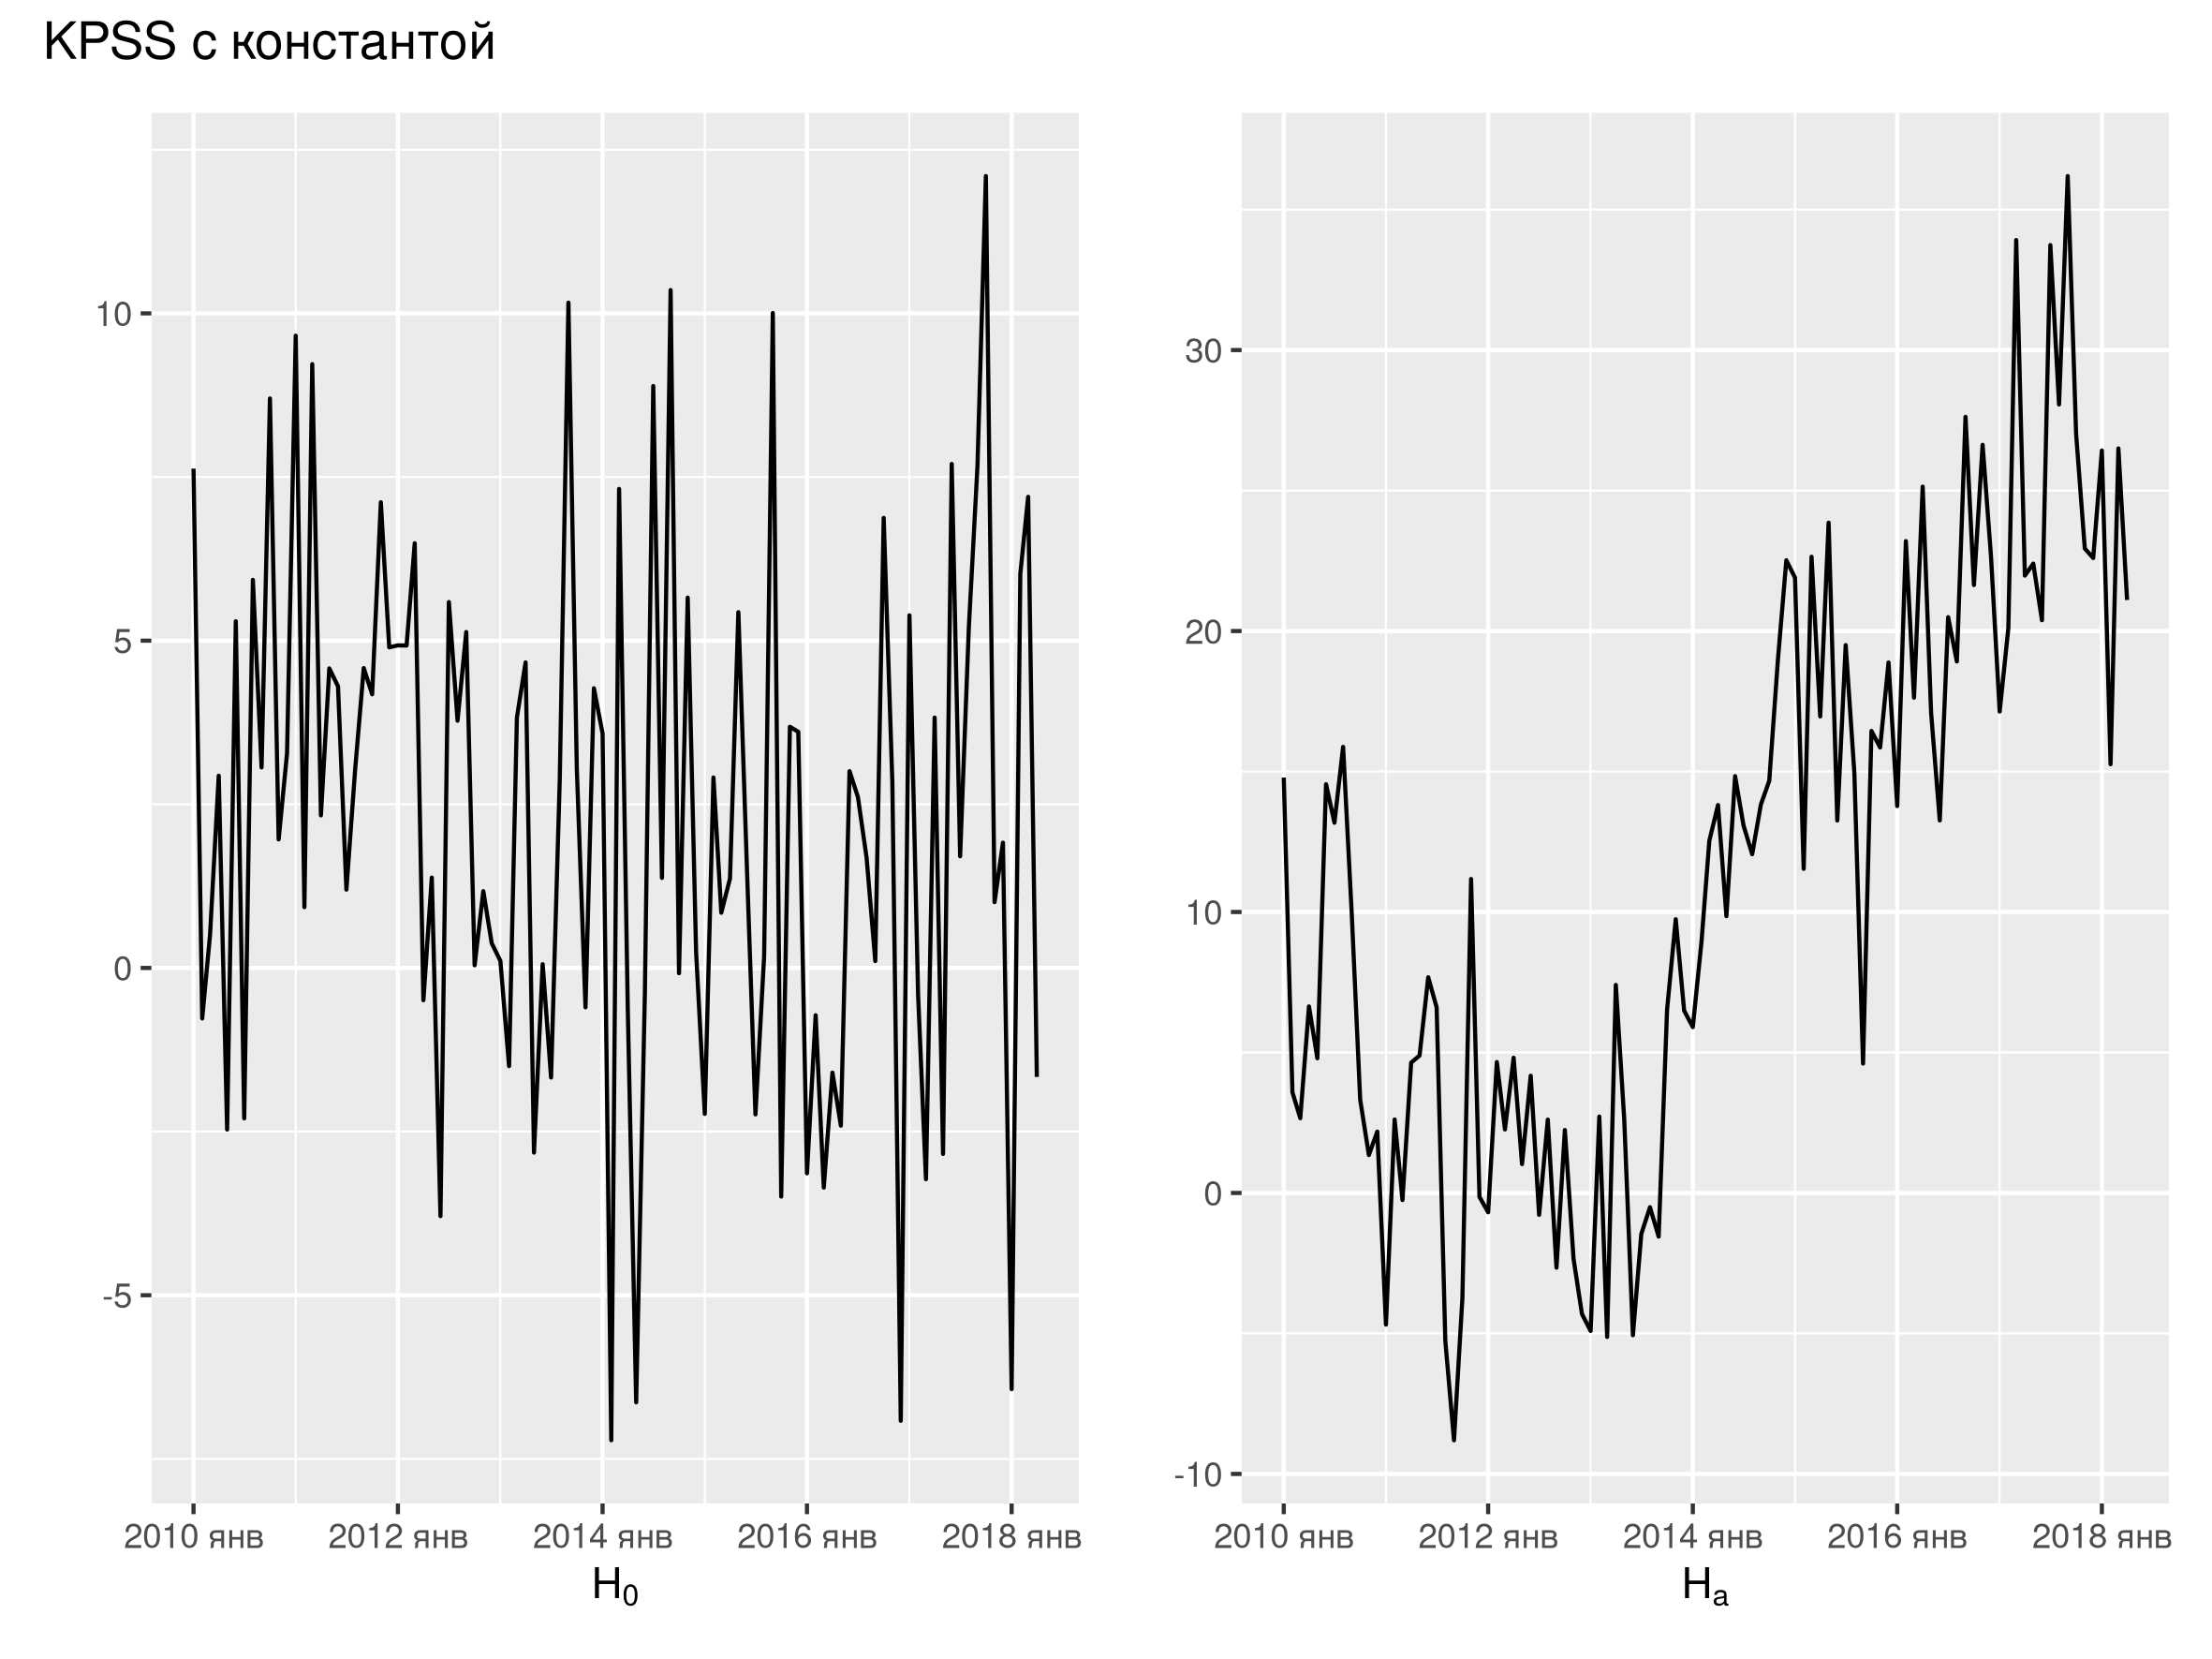
\includegraphics[width=\textwidth]{pictures/om_ts_06-077.png}
  
  \end{frame}
  
  \begin{frame}
    \frametitle{KPSS с константой: алгоритм}
  
    Шаг 1. Оцениваем \alert{регрессию на константу} 
    \[
      \widehat{y_t} = \hat c.  
    \]
  
    \pause
    Шаг 2. Считаем $KPSS$ статистику
    \[
    KPSS = \frac{\sum_{t=1}^T S_t^2}{T^2 \hat \lambda^2},
    \]
    где $S_t$ — накопленная сумма остатков, $S_t = \hat u_1 + \ldots + \hat u_t$,

    а $\hat\lambda^2$ — состоятельная оценка долгосрочной дисперсии. 
  
    \pause
    При верной $H_0$ распределение $KPSS$-статистики стремится к \alert{особому распределению} $KPSS^c$!
  
    \pause 
    Шаг 3. Делаем вывод:
    
    Если $KPSS > KPSS^c$, то $H_0$ отвергается. 
  
  \end{frame}
  
  
  \begin{frame}
    \frametitle{KPSS с трендом}
    \[
      y_t = c + bt + rw_t + x_t,
    \]
  
    \pause
  
    \alert{$H_0$: $rw_t = 0$};
    
    $(x_t)$ — стационарный процесс с $\E(x_t) = 0$;
    
    \pause
  
    \alert{$H_a$: $rw_t = rw_{t-1} + u_t$};

    $rw_0 = 0$;
  
    $(x_t)$ — стационарный процесс с $\E(x_t) = 0$;

    $(u_t)$ — белый шум, независимый с $(x_t)$.
  
    \pause 
  
    В алгоритме будет регрессия \alert{с константой и трендом} и другое распределение $KPSS^{ct}$.
  
  \end{frame}
  
  
  \begin{frame}
    \frametitle{$KPSS$ с трендом: $H_0$ и $H_a$}
    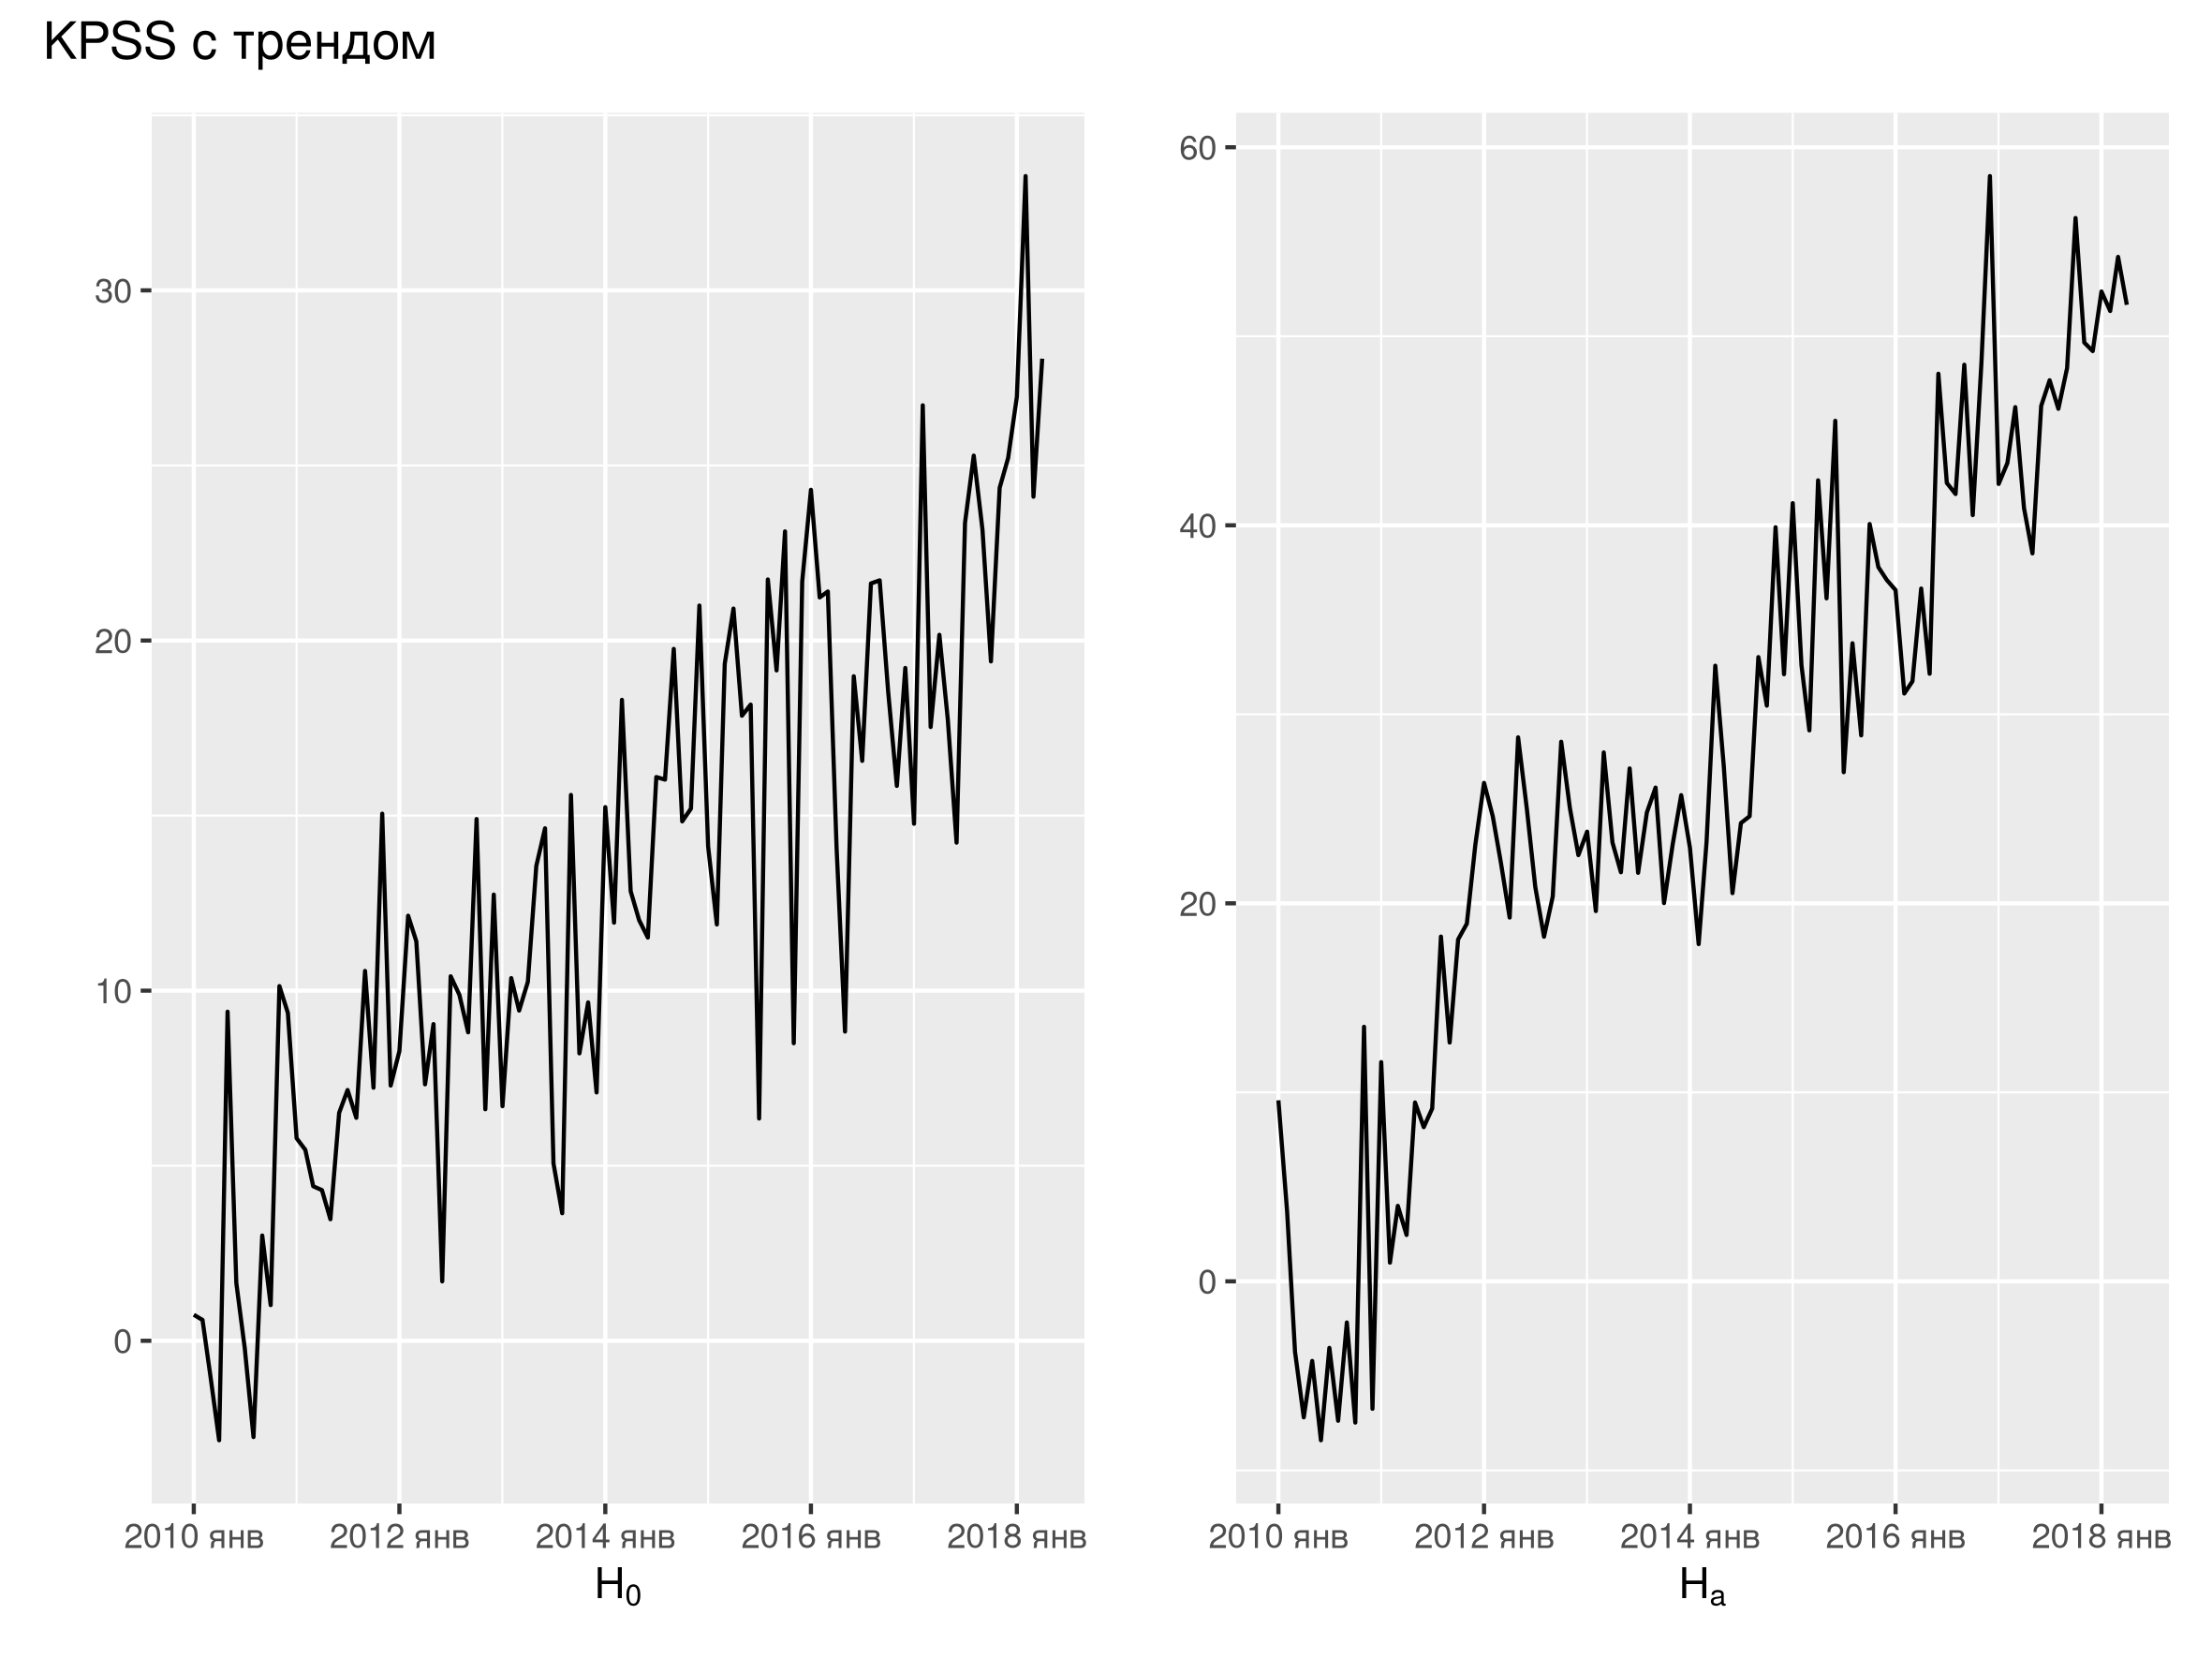
\includegraphics[width=\textwidth]{pictures/om_ts_06-086.png}
  \end{frame}
  
% TODO: сдвинуть A и B и выделить цветом!
  \begin{frame}
    \frametitle{Устоявшаяся терминология:}
    \[
      A. \quad y_t = a + bt + x_t;
    \]

    $(y_t)$ — \alert{стационарный вокруг тренда} (trend stationary).

    $(x_t)$ — стационарный процесс с $\E(x_t) = 0$.

    \pause Рецепт: оценим регрессию $a + bt$ с $ARMA$ ошибками для $(y_t)$.
    \pause 
    \[
      B. \quad y_t = a + \sum_{i=1}^t x_i \text{ или } y_t = a + bt + \sum_{i=1}^t x_i
    \]

    $(x_t)$ — стационарный процесс с $\E(x_t) = 0$.

    $(y_t)$ — \alert{стационарный в разностях} (difference stationary).

    \pause Рецепт: оценим $ARMA$ для $(\Delta y_t)$.

    \pause Оба $(y_t)$ нестационарны!
    
  \end{frame}


  
  \begin{frame}{$KPSS$ тест: итоги}
  
    \begin{itemize}[<+->]
      \item Применим для принятия решения о переходе к $\Delta y_t$.
      \item Есть два варианта теста с разными предпосылками.
    \end{itemize}
  \end{frame}
  
  
  
  